\documentclass[a4j,fleqn,10pt]{jarticle}
\usepackage{katfuji}
\usepackage{amsmath}
\usepackage{txfonts}
\usepackage[symbol*,perpage]{footmisc}
\usepackage[dvips]{graphicx}
\usepackage[usenames,dvipsnames]{xcolor}

% カスタムpackage
\DeclareTextFontCommand{\emph}{\em}
\usepackage{float}
\usepackage[utf8]{inputenc}
\usepackage[T1]{fontenc}
\usepackage{placeins}
\usepackage[subrefformat=parens]{subcaption}
\usepackage{type1cm}
\usepackage{enumitem}
\usepackage{multirow}
\usepackage{plext}
\newcommand{\argmax}{\mathop{\rm arg~max}\limits}
\newcommand{\argmin}{\mathop{\rm arg~min}\limits}
\newcommand{\softmax}{\mathop{\rm softmax}\limits}
\global\long\def\T#1{#1^{\top}}
\newcommand{\cev}[1]{\reflectbox{\ensuremath{\vec{\reflectbox{\ensuremath{#1}}}}}}
\DeclareMathAlphabet{\mathpzc}{OT1}{pzc}{m}{it}
\usepackage{mathtools}
\usepackage{bm}
\usepackage{algpseudocode}
% remove end sentences
\algtext*{EndWhile}
\algtext*{EndIf}
\algtext*{EndFor}

\def\baselinestretch{0.88}

% 図と図の間のスペース
\setlength\floatsep{1truemm}
% 本文と図の間のスペース
\setlength\textfloatsep{5truemm}
% 本文中の図のスペース
\setlength\intextsep{0pt}
% 図とキャプションの間のスペース
\setlength\abovecaptionskip{1truemm}

%-------------------------------------------jtitle and jauthors information
\begin{document}

% 数式の余白調整
\setlength{\abovedisplayskip}{-4pt} % 上部のマージン
\setlength{\belowdisplayskip}{2pt} % 下部のマージン


\jtitle{
  予備実験:GCNによる議論要素の特定
  \\{\large \it 
  Graph Convolutional Networks for Argument Component Identification
}}

\jcontact{
\dag 東京農工大学大学院 工学府
}

\jauthor{森尾 学\dag}

\maketitle

%-------------------------------------------etitle and eauthors information
\footnotetext[0]{\hspace*{-6.5mm}\dag morio@katfuji.lab.tuat.ac.jp}
\footnotetext[0]{\hspace*{-7.5mm} ©藤田桂英研究室. 再配布厳禁.}

%-------------------------------------------document

\section{背景:どこに問題意識を感じているか}
Argument Component Identification (ACI)はArgument Miningにおける最も基礎的なサブタスクである.簡単に言えば,ACIは議論的な文章から「主張」や「前提」になっていそうな部分をトークンレベルで抽出するタスクである\cite{stab2017}.ACIによって抽出された部分はArgument Component (AC)と呼ばれる.

\par
例えば,Essayデータセット\cite{stab2017}(学生が書いたエッセイに対して,Argument Miningのアノテーションを行ったデータセット)には「As a result, it is clear that people can freely express their patriotic feelings during international sports events.」という文章が含まる.この中からACを抽出すると,「it is clear that people can freely express their patriotic feelings during international sports events」となる.

\begin{figure*}[t]
\begin{center}
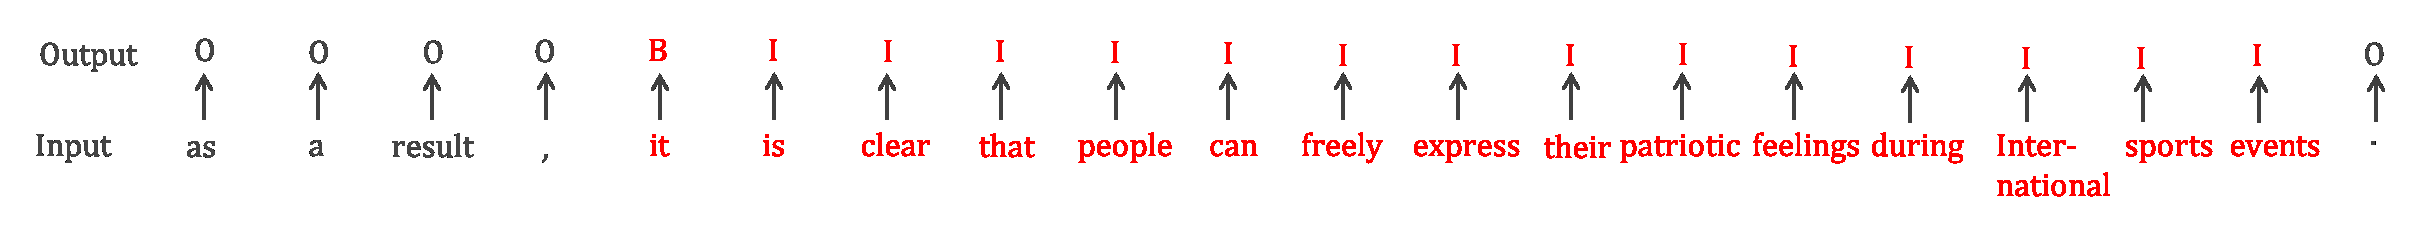
\includegraphics[width=\linewidth]{figure/bio.eps}
\end{center}
\caption{figure/encoding.epsを貼り付けます}
\label{fig:bio}
\end{figure*}

\par
ACの抽出は,系列ラベリングの問題に落とし込める.一般的にはBIOエンコーディングといって,ACの最初のトークンを"B",ACの中のトークンを"I",ACの外のトークンを"O"で表す.図\ref{fig:bio}に,先程のエッセイの例をBIOで可視化したものを示す.

\par
このBIOエンコーディングを行うために,従来とられて来た手法は主に以下の通り:

\begin{itemize}
  \setlength{\parskip}{0cm} % 段落間
  \setlength{\itemsep}{0cm} % 項目間
  \item 特徴ベースのCRF(条件付き確率場)
  \item 双方向LSTM
  \item 双方向LSTM+CRF
  \item 文字レベルCNN+双方向LSTM+CRF
\end{itemize}

\noindent
入力には,単語のBoWやGlove埋め込み表現,品詞埋め込み表現などが用いられてきた.しかし「依存構造」が用いられることは多くなかった.また,ニューラルネットにおいて依存構造解析結果を入力としたアーキテクチャが開発されて来なかった.依存構造とは単語間の係り受けの関係である.本研究では,依存構造解析器によって得られる係り受けを明示的にニューラルネットで扱うことで,ACIのパフォーマンスにどのような影響を与えるかを調べる.


\section{関連研究がどんな貢献をしたか}
あああ


\begin{figure*}[t]
\begin{center}
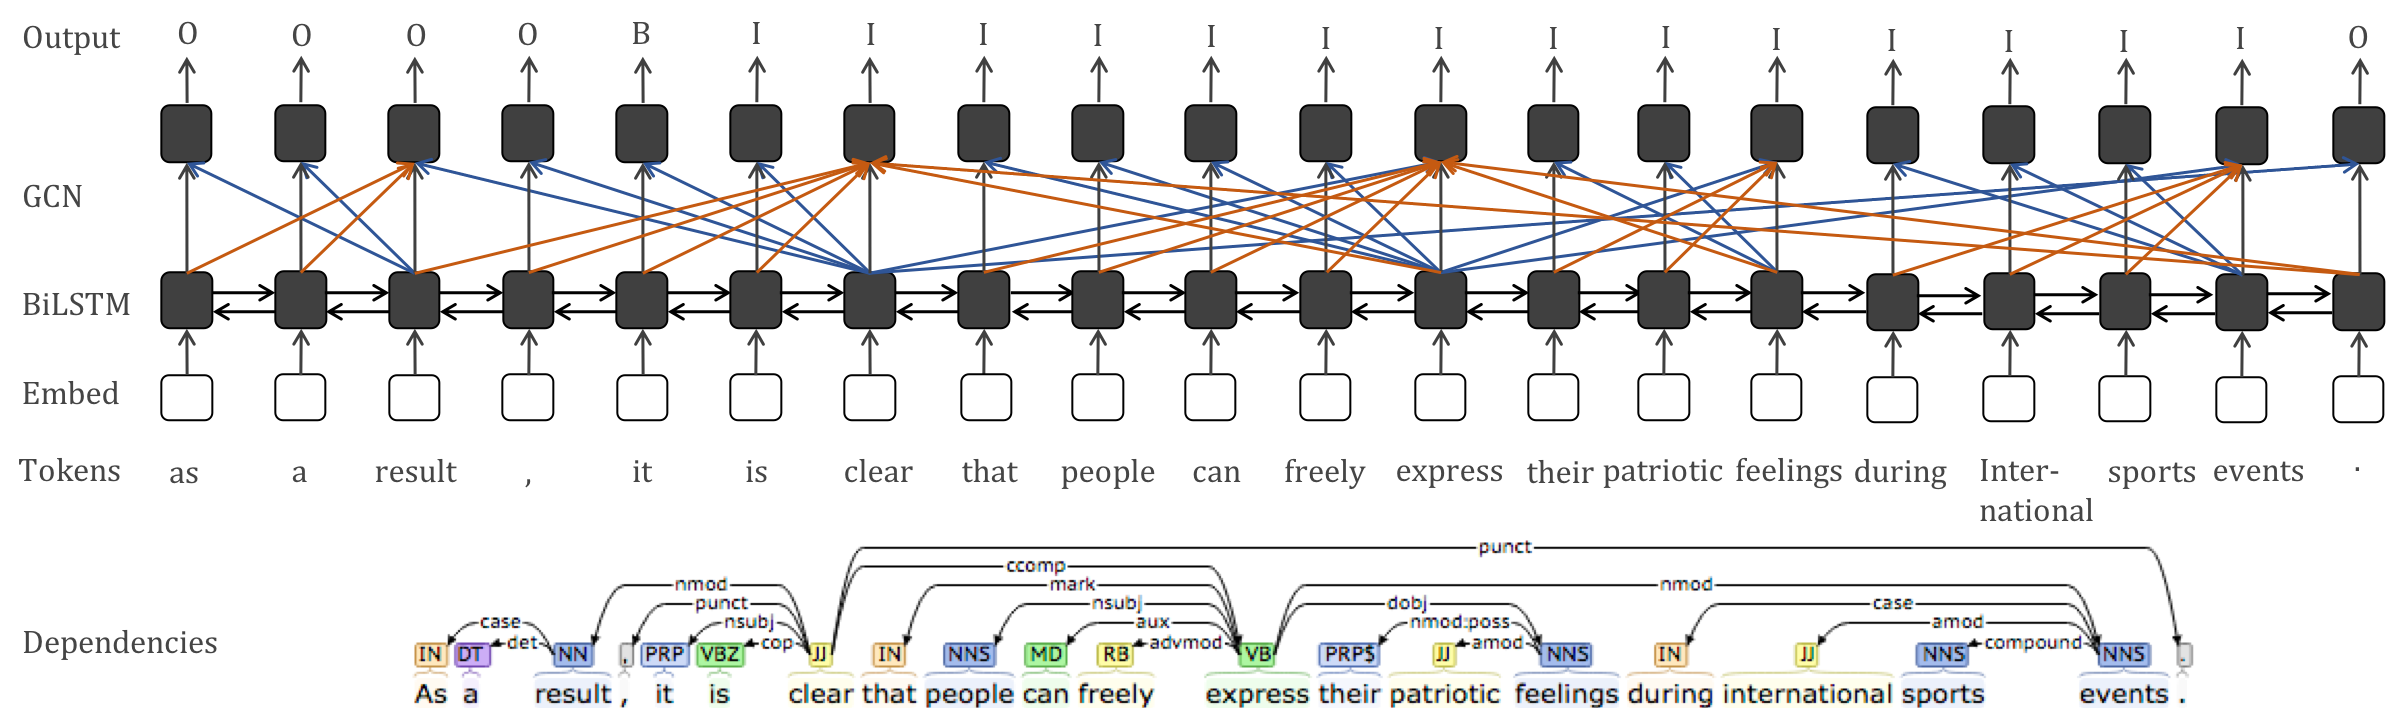
\includegraphics[width=\linewidth]{figure/encoding.eps}
\end{center}
\caption{figure/encoding.epsを貼り付けます}
\label{fig:encoding}
\end{figure*}


\section{提案手法}
ううう

\section{実験結果から何がわかったか}
えええ


\footnotesize
\bibliographystyle{jplain}
\bibliography{katfuji}

\end{document}
